\section{Security}

\subsection{Role Access Management}
The application is a fusion of two distinct projects that share common code. Each project includes functionalities tailored for two different roles: staffing and HR. Therefore, we need to secure our API not only with authentication but also based on the role of the current user. Additionally, some functionalities are also restricted to privileged users such as managers or admins. 


\subsubsection{Open Policy Agent}

Open Policy Agent (OPA)[ici] is an open-source solution that enables us to define, enforce, and manage policies for our systems and services. OPA is designed to be flexible and high-performance, with minimal processing requirements (RAM, CPU ...), allowing easy integration into different environments and independence from the programming language used. 


\paragraph{Deployment}: OPA needs to run as a separate service or server. This requires deploying a new server in the cloud, though OPA's lightweight processing footprint ensures it remains almost invisible in terms of resource consumption and so it is a waste of money for our use case. It could also be installed using Docker but this is currently not possible in our platform. Another solution would be to have a standalone binary that can be run directly inside our application. However this last one requires to allow command execution and is dependant on the OS used, this make it not possible for us. 


\paragraph{Functionning}: Once deployed, OPA controls access using a list of rules written in Rego, its declarative policy language. These rules are evaluated to make policy decisions, enabling fine-grained access control across various services and systems. OPA evaluates incoming requests against these rules and returns a decision, ensuring that access is granted or denied based on predefined policies. 


\paragraph{Integration}: To integrate OPA, after running it as another service we will communicate with thanks to request where we can send anything as JSON for our rules. For this, in our spring boot application we use filters that will handle all the requests and redirect it into OPA. Based on the return it will give, will either pursue the processing of the request or denied the access of the end point to the user. 


\begin{figure}[H]
	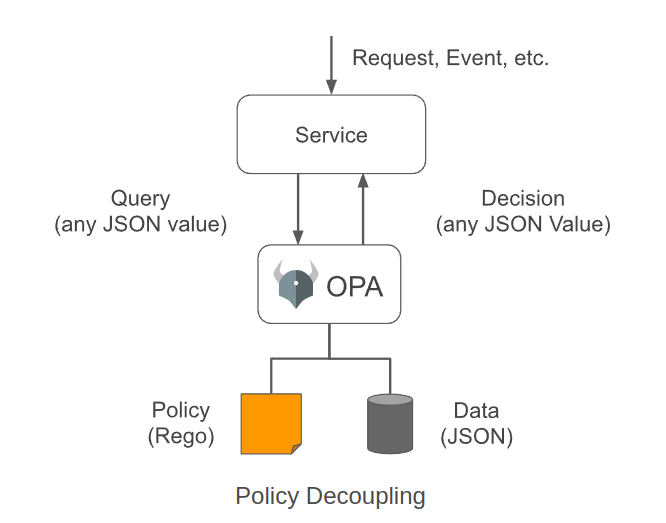
\includegraphics[width=150mm]{Image/OPA}
	\caption{OPA deployment}
	\label{fig:OPA deployment}
\end{figure}


\subsubsection{Cache management}

Another approach has been explorated and then chosen. Instead of deploying complexe services and using special policies we can indeed build a table that will contains our rules. This one is more efficient as it is accessible directly in the application and need no communication.

\begin{center}
	\begin{tabular}{| c | c | c |}
		\hline
		method & end point & roles allowed\\ \hline
		GET & /employees/\{id\} & HR, STAFFING\\
		\hline
	\end{tabular}
\end{center}

Since access needs to be checked for each request, processing can become intensive for this simple task. To optimize these access checks, we can use a caching mechanism that reduces the computational loading for evaluating access decisions by storing the table directly in the cache. This one enhances the performance by quickly serving subsequent requests. 
Indeed, we can manage the cache to improve it again. 
Instead of caching the entire table and searching through it for access control decisions, we can optimize both space and processing by caching the results of the function itself. With a well-structured approach, we can store the function's output based on its parameters. By using a long expiration policy, we reduce the need to reprocess these functions frequently. Indeed, once the function has run and its result is cached, subsequent requests with the same parameters can retrieve the result directly from the cache, eliminating the need to rerun the function.


\paragraph{Deployment}: the cache is directly managed inside the application, we don't need to do anything else that configuring the name, the type that will be stored and a unique key to access an element. Finally the time to leave is also configurable. 


\paragraph{Functionning}: Usually, the cache is used to store complex objects to avoid redundant computations and expensive operations. By caching these complex objects, we reduce the need for recalculating or refetching data, which enhances performance and efficiency.  
In our case, the cache helps by directly storing access check results. Indeed we have a long list where we need to check if a role has the access to a certain end point. Searching in this list at each request may be not efficient and not interessing for us. For this reason, we directly cache the result of a function that will search inside this list. Whenever we try again with the same parameters, instead of looking inside this list the cache will directly give us the answer. 



\paragraph{Integration}: To integrate this caching-based access management method, we use a filter[ici] that intercepts requests after authentication. This filter extracts user information, including the current role, from the authentication token. Based on the user's role and the requested endpoint, the filter checks the access permissions stored in the cache. This allows the system to efficiently determine whether to grant or deny access to the requested end point. 
